{\let\clearpage\relax \chapter{Evaluation}\label{ch:eval}}
In this section, we evaluate the performance of literature search queries based on the introduced metrics. This evaluation serves as a foundation for developing tools that can potentially generate automatic literature search queries in the future. It is crucial to note that the objective of this evaluation is not to only assess the SQW tool itself, but rather to evaluate any arbitrarily generated literature search query. Thus, the focus is solely on the quality of the query, independent of the method by which it was generated.

\vspace*{.5cm}

\section{Experimental Setup}
The curated dataset is constructed using two distinct methods to identify core publications: Bibliometric Analysis (14 topics) and Systematic Literature Review (7 topics), as illustrated in \autoref{fig:dataset-overview}. For the SLRs, the original queries used by the researchers are available. Consequently, we conduct two main experiments. In both experiments we use Dimensions.ai to retrieve all required data. The retrieval process relies on their default relevance-based sorting method, which ranks publications based on the number of keyword matches between the title-abstract and the provided query.

The first experiment involves all 21 topics from both the SLRs and BAs, where we compare a baseline query against a query generated by the SQW. The baseline query consists of the exact topic name, passed into the search engine in a non-exact search fashion. For instance, the query \textit{Soft Robotics} retrieves publications containing both words in their title or abstract, even if they do not appear consecutively.

The predicted query, however, is semi-automatically generated using the SQW tool. This process begins by providing the baseline query as input, which generates a list of keywords. These keywords are then manually sorted by the author into specific or general categories, as described in \autoref{fig:sqw-stage1}. The overarching topic is derived from the topic itself; for example, in the case of \textit{Soft Robotics}, the overarching keyword \textit{Robot} is used. In some cases, the resulting queries produced excessively large results (>100k publications). To address this, keywords were filtered to limit the results to a maximum of 50k publications, balancing evaluation cost and processing speed. Importantly, the baseline query is always included in the predicted query. This ensures that recall is at least as high for the predicted query as for the baseline, making the primary goal of the evaluation to determine whether the expanded query retrieves more core publications than the baseline without becoming overly general by retrieving irrelevant publications.

The second experiment focuses exclusively on the 7 SLR topics. It uses the exact baseline queries and results from the first experiment but compares them to SLR queries manually crafted by experts in the field rather than those generated by the SQW. These SLR queries are designed with well-defined research questions aimed at retrieving the most relevant publications that help tackle these exact questions.

\section{Results}
Using the data from the first experiment, we computed all the metrics, namely: Cosine Precision, Clustering Precision, MVEE Precision, Hull Precision, Recall, and the F2 score for each precision metric, as shown in Figure \autoref{fig:all-metrics-1}. When examining the precision metrics, the clustering precision distinctly stands out due to its high value in certain cases, which can be directly attributed to low recall. This recall issue is also evident in some instances for the MVEE and Hull metrics, such as the baseline for \textit{Drones in Agriculture}, where they are set to 0 because fewer than three retrieved core publications are available, which is the minimum number required to define a plane.

\begin{figure}[!b]
	\hspace*{-1cm}	
	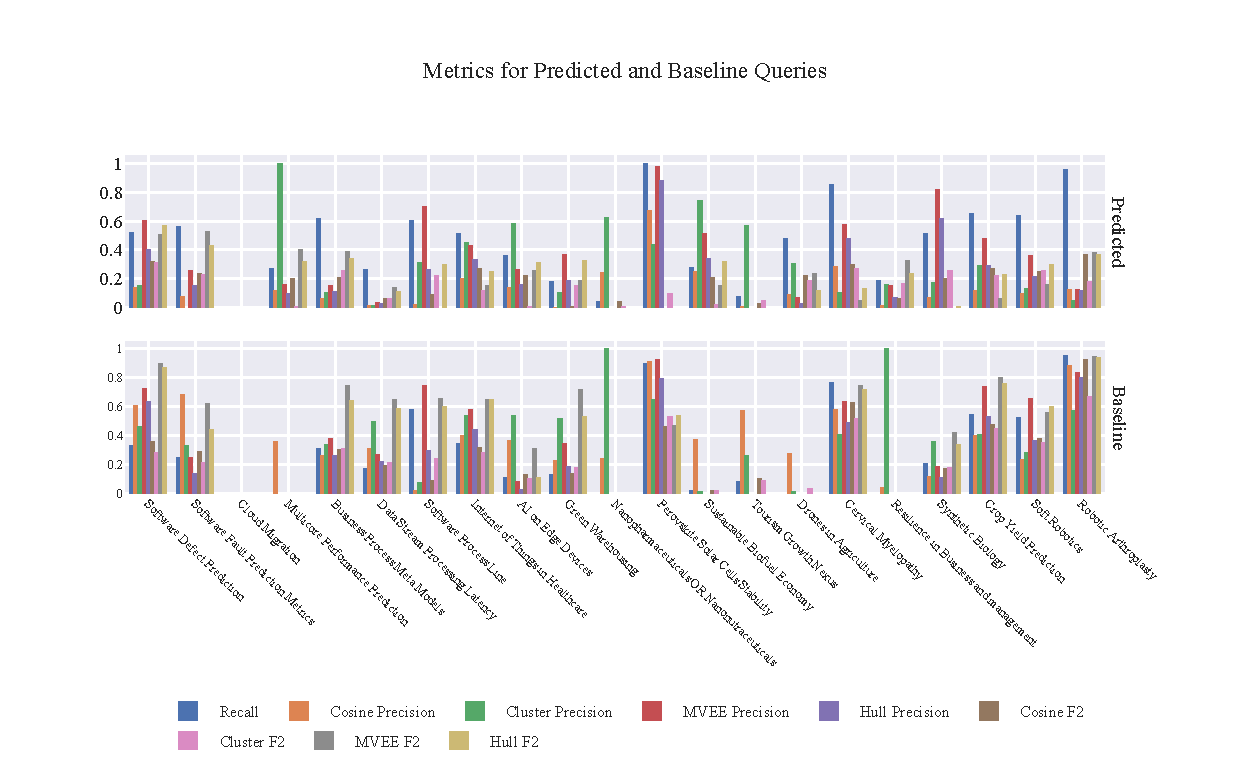
\includegraphics[scale=0.45]{pics/all-metrics-1.pdf}
	\caption[Evaluation: Experiment 1]{This figure shows the results of the first experiment across all the datasets. Initially, the issue with the clustering, MVEE, and Hull precision metrics becomes apparent in cases such as \textit{Cloud Migration} and \textit{Multicore Performance Prediction}, where the value is 0. This occurs due to a recall that is <3 for MVEE and Hull and recall of 0 for the clustering. On the other-hand the impact of the crafted F2 score is particularly evident in cases like \textit{Robotic Arthroplasty}, where the baseline score is very high. Conversely, for the predicted query, which retrieves more publications but maintains the same recall, the score is significantly lower.}\label{fig:all-metrics-1}
\end{figure}

A strong correlation is observed between cosine precision and the MVEE and Hull methods, despite relying solely on UMAP embeddings to define the enclosing shapes. This highlights the robustness of these approaches in identifying semantically relevant publications. Additionally, we have two special case topics that had 0 recall, namely \textit{Cloud Migration} and \textit{Multicore Performance Prediction}. As expected, these resulted in a 0 across the board except for the cosine similarity, since it does not require any of the retrieved core publications to exist in order to compute. Instead, it only relies on the pre-computed average embeddings of the core publications.

Considering the F2 score, a notable example of the impact of overly large queries without any recall improvement is \textit{Robotic Arthroplasty}. Both the baseline and predicted queries achieved a recall of 0.957, but the expanded predicted query from the SQW retrieved significantly more results overall. Specifically, the predicted query retrieved 22,892 publications, of which only 2,834 were relevant based on cosine similarity. In contrast, the baseline query retrieved 2,151 documents, with 1,904 classified as relevant. This demonstrates how an excessively large query can dilute the precision without improving recall or the number of relevant documents retrieved.

In \autoref{fig:eval1_results}, we can better interpret the results of the first experiment by examining the differences between the scores of the predicted query and the baseline. Here, positive values indicate that the predicted query performs better, while negative values show that the baseline outperforms the predicted query. 

As expected, the predicted query consistently achieves similar or better recall across all topics due to the inherent nature of the SQW. However, when evaluating precision, it is evident that the broader queries generated through query expansion often degrade the performance of the model. This effect is particularly visible in the F2 scores, where the increased number of irrelevant publications impacts the balance between recall and precision.

While the SQW demonstrates advantages in terms of recall, its over-expansion often leads to excessive noise in the results. This trade-off is especially clear for topics with a significant drop in precision or F2 scores due to the broader query scope.

\begin{figure}
	\hspace*{-.8cm}	
	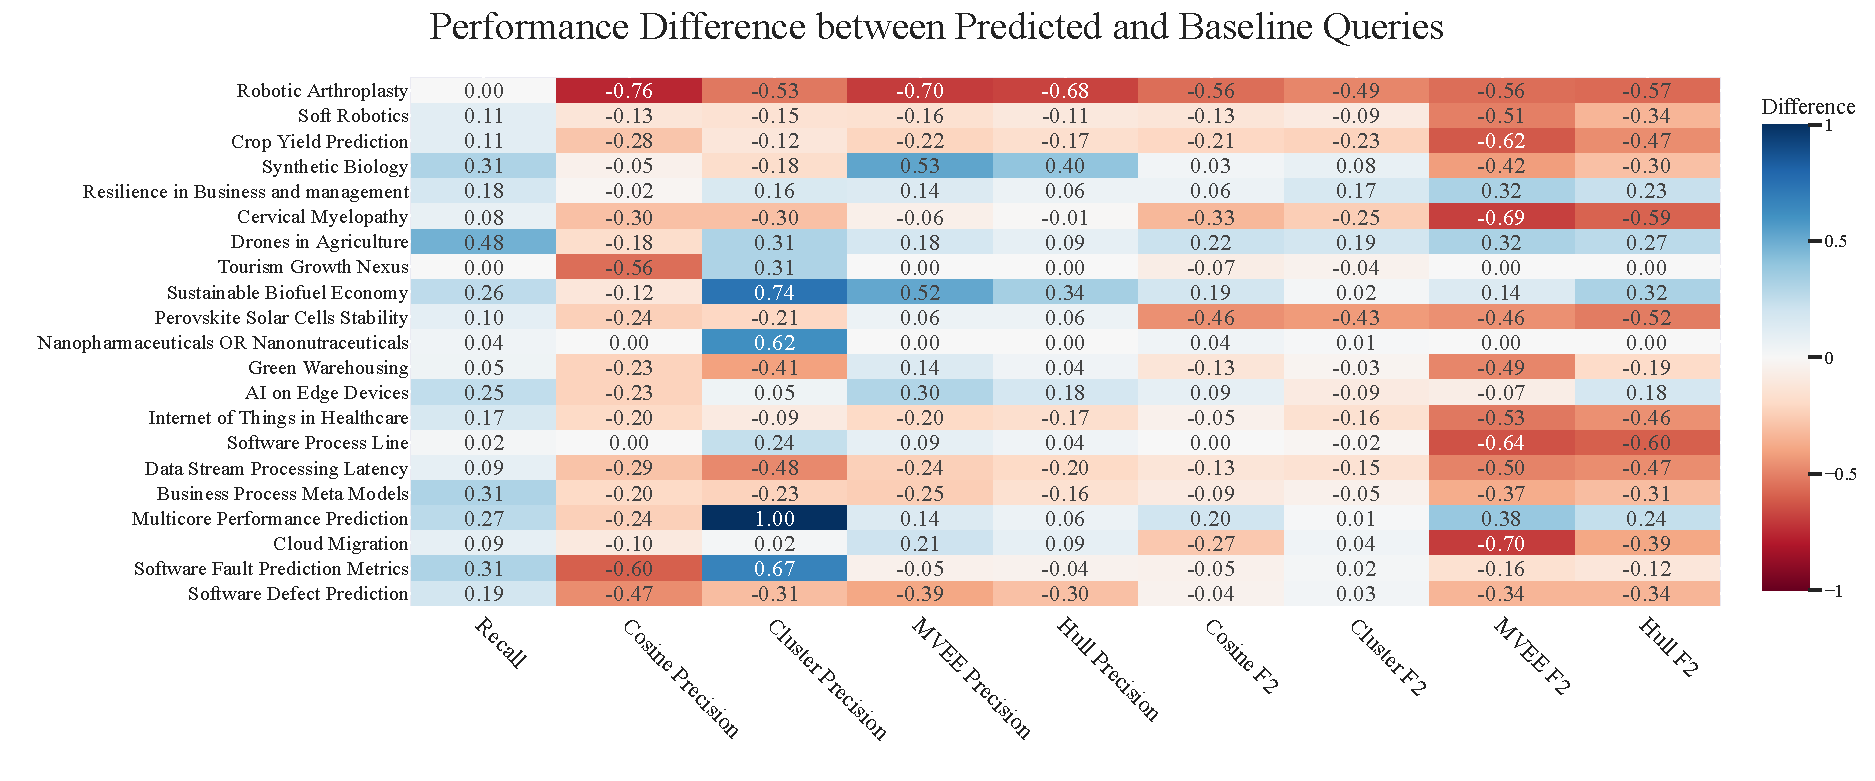
\includegraphics[scale=0.45]{pics/eval1_results.pdf}
	\caption{In this figure we can see the difference in values between the predicted query from the SQW and the baseline, whereby a negative value means that the baseline is better. As anticipated we at least always achieve a similar recall, but in most cases, the SQW yields better recall. However, it severely suffers in precision. When looking at the F2 value, we can see that the tool only notably outperforms the baseline on the three topics \textit{Drones in Agriculture}, \textit{Sustainable Bio Fuel Economy}, and \textit{Multicore Performance Prediction}, whereas it shows a clear disadvantage on the topics \textit{Perovskite Solar Cells Stability}, \textit{Robotic Arthroplasty}, and \textit{Cervical Myelopathy}.}
	\label{fig:eval1_results}
\end{figure}

The results of the second experiment, which compare the actual search queries used to identify the core publications in the SLRs, have yielded surprising yet explainable outcomes. It is important to re-emphasize that the queries initially used for the SLRs were adapted to fit dimension's query criteria and were only applied to search the title and abstract. In contrast, the original queries were utilized across a variety of search indices, such as title, abstract, full text, and sometimes full data for specific fields, which is a form query fine-tuning that is search engine specific. Therefore, it is important to note that the results will always be search engine dependent, which, in this case, is dimensions.ai.

As shown in \autoref{fig:all-metrics-2}, the results of the SLR queries are not as anticipated, particularly since they were expected to yield high recall. This discrepancy arises from the queries' reconstruction and adaptation to fit dimensions' criteria. The performance difference between the SLR queries and the baseline can be observed in \autoref{fig:eval2_results}. Overall, the baseline and the SLR queries performed on nearly equal footing, with two topics favoring the SLR and three favoring the baseline. 

Interestingly, in case where the recall of the baseline significantly outperformed the SLR, namely \textit{Software Fault Prediction Metrics}, the cosine precision was drastically lower. This results in an unwanted behavior which can be interpreted by the cosine-F2 score being 0, indicating that the recall gain was of no value due to the excessive number of irrelevant retrieved publications.


\begin{figure}	
	\centering
	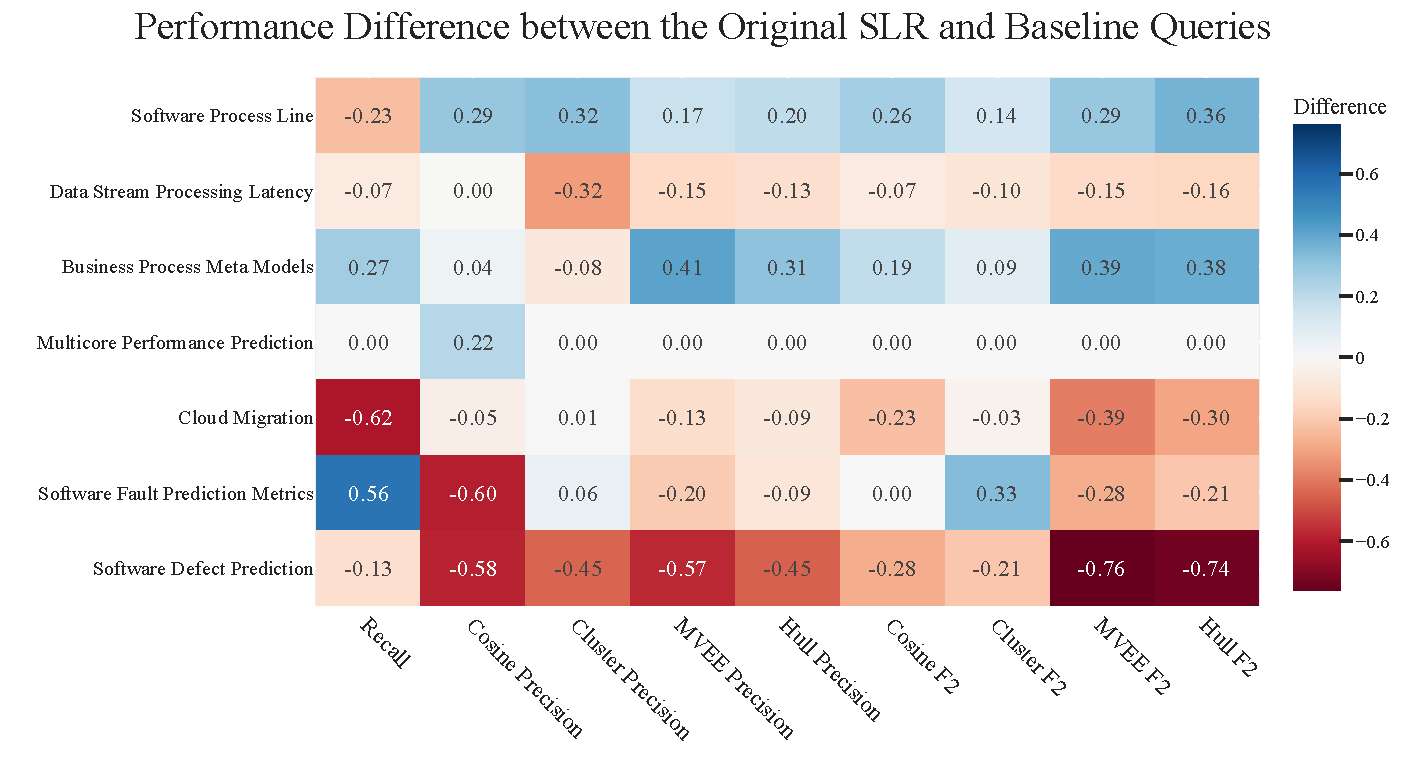
\includegraphics[scale=0.45]{pics/eval2_results.pdf}
	\caption{This figure displays the metric values difference between the original SLR query and the baseline, where a negative value indicates that the baseline performs better.}
	\label{fig:eval2_results}
\end{figure}

\section{Discussion}

The primary goal of this work was to determine the quality of literature search queries, emphasizing recall, which is widely regarded as an essential measure in the research community. However, precision has historically been less emphasized due to the intrinsic nature of literature search queries, which tend to favor comprehensiveness over specificity. By developing multiple metrics to evaluate the relevance of publications in a semantic space, we successfully integrated precision into the evaluation framework by introducing semantic precision.

To calculate semantic precision, we employed four metrics: semantic cosine, clustering, MVEE, and Hull precision. Each metric demonstrated distinct advantages and limitations. Initially, we hypothesized that the cosine similarity threshold should correspond to the least similar core publication. However, in certain cases, sacrificing a core publication to substantially reduce the number of irrelevant publications proved more beneficial in terms of the F2 score. Consequently, we adopted an empirical threshold estimated by maximizing the F2 score across all topics.

For Convex Hull and MVEE, we first tested their performance using the original embeddings in their high-dimensional space. However, these metrics consistently overestimated precision, often exceeding 50\%. This discrepancy is likely due to the curse of dimensionality, which complicates the construction of accurate ellipsoids or hulls in high-dimensional spaces, possibly reflecting limitations in the embedding construction process. This observation led to the decision to switch to UMAP embeddings, which offer a reduced dimensionality and improved computational feasibility. However, while UMAP embeddings show potential, the exact amount of semantic value lost compared to the original high-dimensional embeddings remains unclear.

A common issue for clustering, MVEE, and Hull methods lies in their dependency on recall. Semantic clustering requires at least two core publications, and performance improves with more core publications as the clustering process narrows the focus on relevant publications. This limitation becomes problematic when the viable core publications count is less than two. Similarly, MVEE and Hull methods necessitate at least three core publications to construct a plane capable of enclosing other potentially relevant publications. In contrast, cosine similarity only requires the pre-computed mean embedding of the core publications and a similarity threshold. This independence from recall allows cosine similarity to determine relevance even when recall is minimal, making it a more robust metric in cases of sparse core publications.





